\pagebreak{}
\section{Applets}
\begin{verbatim}

import java.awt.*;
import java.applet.*;
public class Sum extends Applet {

    TextField text1,text2;

    public void init()
    {
        text1 = new TextField(8);
        text2 = new TextField(8);
        add(text1);
        add(text2);
        text1.setText("");
        text2.setText("");
    }

    public void paint(Graphics g)
    {
        int x = 0, y = 0, z = 0;
        String s1,s2,s;
        g.drawString("Input a number in the textbox", 10, 50);
        try {
            s1 = text1.getText();
            x = Integer.parseInt(s1);
            s2 = text2.getText();
            y = Integer.parseInt(s2);

        }
        catch (Exception ex) {

        }
        z = x + y;
        s = String.valueOf(z);
        g.drawString("The sum is:", 10, 75);
        g.drawString(s, 100, 75);
    }

    public boolean action(Event event, Object object)
    {
        repaint();
        return true;
    }
}
\end{verbatim}
\section*{Output}
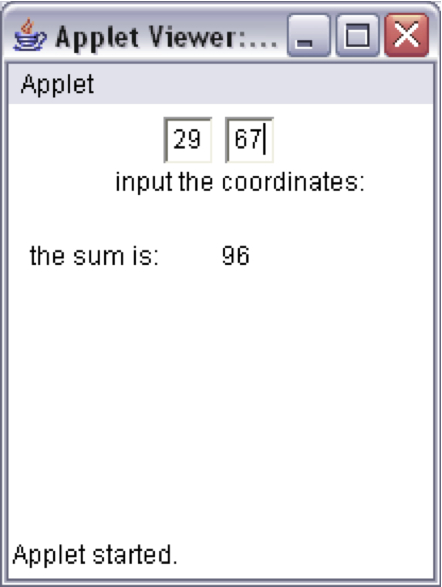
\includegraphics{applet}